\documentclass[aspectratio=169, 10pt]{beamer}

\usetheme{metropolis}
\usepackage{booktabs}
\usepackage{graphicx}
\usepackage{multirow}
\usepackage{array}
\usepackage{appendixnumberbeamer}
\usepackage{caption}
\usepackage{amsmath,amssymb}
\usepackage[backend=biber]{biblatex}
\addbibresource{references.bib}

% ── Colour palette ──────────────────────────────────
\definecolor{PrimaryBlue}{HTML}{1A73E8}
\definecolor{AccentTeal}{HTML}{00897B}
\definecolor{DarkBg}{HTML}{23272F}
\definecolor{LightGray}{HTML}{F5F5F5}

\setbeamercolor{palette primary}{bg=PrimaryBlue}
\setbeamercolor{frametitle}{bg=PrimaryBlue, fg=white}
\setbeamercolor{title separator}{fg=AccentTeal}
\setbeamercolor{progress bar}{fg=AccentTeal, bg=LightGray}
\setbeamercolor{block title}{bg=AccentTeal, fg=white}
\setbeamercolor{alerted text}{fg=AccentTeal}

\setbeamerfont{title}{series=\bfseries, size=\Large}
\setbeamerfont{frametitle}{series=\bfseries}

% ── Meta ────────────────────────────────────────────
\title{Exploring Human Steering Performance\\on Complex 3D Paths}
\subtitle{Prototype Design and Construction for a Human-Centered Evaluation System}
\author{
  Yousuf Ibne Kamal Niloy \and
  Samnun Azfar \and
  Anika Farzana \and
  Yousef Fuad Ahmed Al-Khasheb
}
\institute{
  Department of Computer Science and Engineering\\
  Islamic University of Technology (IUT), OIC
}
\date{CSE 6275 / CSE 6391: AHCI --- Assignment 2}

% ═══════════════════════════════════════════════════
\begin{document}

% ── 1  Title ────────────────────────────────────────
\begin{frame}[plain]
  \titlepage
\end{frame}

% ── 2  Outline ──────────────────────────────────────
\begin{frame}{Outline}
  \tableofcontents
\end{frame}

% ━━━━━━━━━━━━━━━━━━━━━━━━━━━━━━━━━━━━━━━━━━━━━━━━━
\section{Introduction}
% ━━━━━━━━━━━━━━━━━━━━━━━━━━━━━━━━━━━━━━━━━━━━━━━━━

% ── 3  Background ───────────────────────────────────
\begin{frame}{Background \& Motivation}
  \begin{itemize}
    \item \textbf{Steering Law} extends Fitts' Law to trajectory-based tasks:\\
          $MT = a + b \cdot \dfrac{L}{W}$
    \item Modern systems increasingly involve \alert{complex 3D environments}:\\
          VR, simulation training, 3D design, robotic teleoperation
    \item Existing models focus on 2D or simple straight 3D paths
    \item Path \emph{curvature} and \emph{complexity} significantly affect performance
    \item \textbf{Human-Centered Machine Learning (HCML)} aims to model and support
          human behaviour while preserving transparency and user control
  \end{itemize}
\end{frame}

% ── 4  Objectives ───────────────────────────────────
\begin{frame}{Objectives \& Contributions}
  \textbf{Objectives}
  \begin{enumerate}
    \item Port Chen et.\ al's empirical evaluation of a modified Fitts' law to 3D curves \cite{chen2025curves}
    \item Design and construct a \alert{high-fidelity prototype} in Unity3D for 3D curve tracking experiments
    \item Enable researchers to configure curve parameters and collect accurate steering data
  \end{enumerate}

  \vspace{0.5em}
  \textbf{Key Contributions}
  \begin{itemize}
    \item A working Unity3D prototype for toroidal curve tracking
    \item Parameterised curve generation with 6 coefficients (3 sine + 3 cosine)
    \item Crosshair-based interaction with time-tracking data export
  \end{itemize}
\end{frame}

% ── 5  From Requirements to Design ─────────────────
\begin{frame}{From Requirements to Design}
  \textbf{Assignment 1 Recap}
  \begin{itemize}
    \item Identified 5 stakeholder personas and 5 aligned usage scenarios
    \item Specified 12 functional, 8 non-functional, and 4 data/environmental requirements
    \item Key findings: need for standardised 3D path representations, configurable experiments, and reproducible data
  \end{itemize}

  \vspace{0.5em}
  \textbf{Design Direction}
  \begin{itemize}
    \item Prototype translates these requirements into a concrete, testable system
    \item Focus on \alert{accurate data collection} over aesthetic user interaction goals
    \item Curves must remain consistent and trackable across experimental conditions
  \end{itemize}
\end{frame}

% ━━━━━━━━━━━━━━━━━━━━━━━━━━━━━━━━━━━━━━━━━━━━━━━━━
\section{Related Work \& Design Inspirations}
% ━━━━━━━━━━━━━━━━━━━━━━━━━━━━━━━━━━━━━━━━━━━━━━━━━

% ── 6  Related Work ─────────────────────────────────
\begin{frame}{Related Work \& Theoretical Background}
  \begin{columns}[T]
    \begin{column}{0.48\textwidth}
      \textbf{Steering Law Foundations}
      \begin{itemize}
        \item Accot \& Zhai (1997): trajectory-based movement model \cite{accot1997beyond}
        \item Extensions for curvature and path complexity
        \item Limited 3D validation \cite{liu2011revisiting}
      \end{itemize}

      \vspace{0.6em}
      \textbf{3D Curve Porting}
      \begin{itemize}
        \item Chen \& Fels (2025): empirical evaluation for curved paths \cite{chen2025curves}
        \item Our work extends this from 2D to 3D toroidal surfaces
      \end{itemize}
    \end{column}
    \begin{column}{0.48\textwidth}
      \textbf{Prototyping in HCI}
      \begin{itemize}
        \item Iterative design and early usability testing \cite{sharp2019interaction}
        \item Goal-directed design grounded in personas \cite{cooper2014aboutface}
      \end{itemize}

      \vspace{0.6em}
      \textbf{HCAI Principles}
      \begin{itemize}
        \item Transparency, explainability, human oversight \cite{shneiderman2022hcai}
        \item Guidelines for Human-AI Interaction \cite{amershi2019guidelines}
      \end{itemize}
    \end{column}
  \end{columns}
\end{frame}

% ━━━━━━━━━━━━━━━━━━━━━━━━━━━━━━━━━━━━━━━━━━━━━━━━━
\section{Design Goals \& HCAI Principles}
% ━━━━━━━━━━━━━━━━━━━━━━━━━━━━━━━━━━━━━━━━━━━━━━━━━

% ── 7  Design Goals ─────────────────────────────────
\begin{frame}{Design Goals}
  \begin{columns}[T]
    \begin{column}{0.48\textwidth}
      \textbf{Data Collection Goals}
      \begin{itemize}
        \item \textbf{Accuracy:} Millisecond-precision timing of curve tracking
        \item \textbf{Reproducibility:} Deterministic curve generation from coefficients
        \item \textbf{Configurability:} Adjustable curve parameters via UI sliders
        \item \textbf{Consistency:} Curves must be trackable and well-formed across all parameter ranges
      \end{itemize}
    \end{column}
    \begin{column}{0.48\textwidth}
      \textbf{Usability Goals}
      \begin{itemize}
        \item \textbf{Learnability:} Minimal instruction needed for participants
        \item \textbf{Low Cognitive Load:} Crosshair-based tracking with clear visual feedback
        \item \textbf{Researcher Control:} Experiment setters configure curves via sliders
        \item \textbf{Data Integrity:} Automatic time logging and export
      \end{itemize}
    \end{column}
  \end{columns}
\end{frame}

% ── 8  HCAI Principles ─────────────────────────────
\begin{frame}{Human-Centered AI Principles in the Prototype}
  \begin{itemize}
    \item \textbf{Transparency:} All curve parameters and timing data are fully visible and exportable --- no hidden computations
    \item \textbf{Human Oversight:} The researcher maintains full control over experiment configuration; no automated adaptation during trials
    \item \textbf{Explainability:} Curve generation is based on an explicit mathematical formula; results are directly interpretable
    \item \textbf{Reliability:} Deterministic rendering from the same coefficients ensures reproducible experimental conditions
    \item \textbf{Ethical Data Handling:} Trial data is stored locally with no personally identifiable information
  \end{itemize}
\end{frame}

% ━━━━━━━━━━━━━━━━━━━━━━━━━━━━━━━━━━━━━━━━━━━━━━━━━
\section{Conceptual Design}
% ━━━━━━━━━━━━━━━━━━━━━━━━━━━━━━━━━━━━━━━━━━━━━━━━━

% ── 9  System Overview ──────────────────────────────
\begin{frame}{System Overview}
  \begin{columns}[T]
    \begin{column}{0.65\textwidth}
      \textbf{Core Concept}
      \begin{itemize}
        \item A \alert{toroidal curve} is generated on a torus surface in 3D space
        \item The curve is defined by a circle equation plus a sinusoidal height component with 6 adjustable coefficients
        \item A \textbf{crosshair} tracks along the curve; the user drags to follow the path
        \item The system records \textbf{completion time} for each trial
      \end{itemize}

      \vspace{0.5em}
      \textbf{Two User Roles}
      \begin{itemize}
        \item \textbf{Experiment Setter:} Uses sliders to generate curves with different parameters
        \item \textbf{Participant:} Tracks the curve by dragging along the toroidal path
      \end{itemize}
    \end{column}
    \begin{column}{0.35\textwidth}
      \vspace{1cm}
      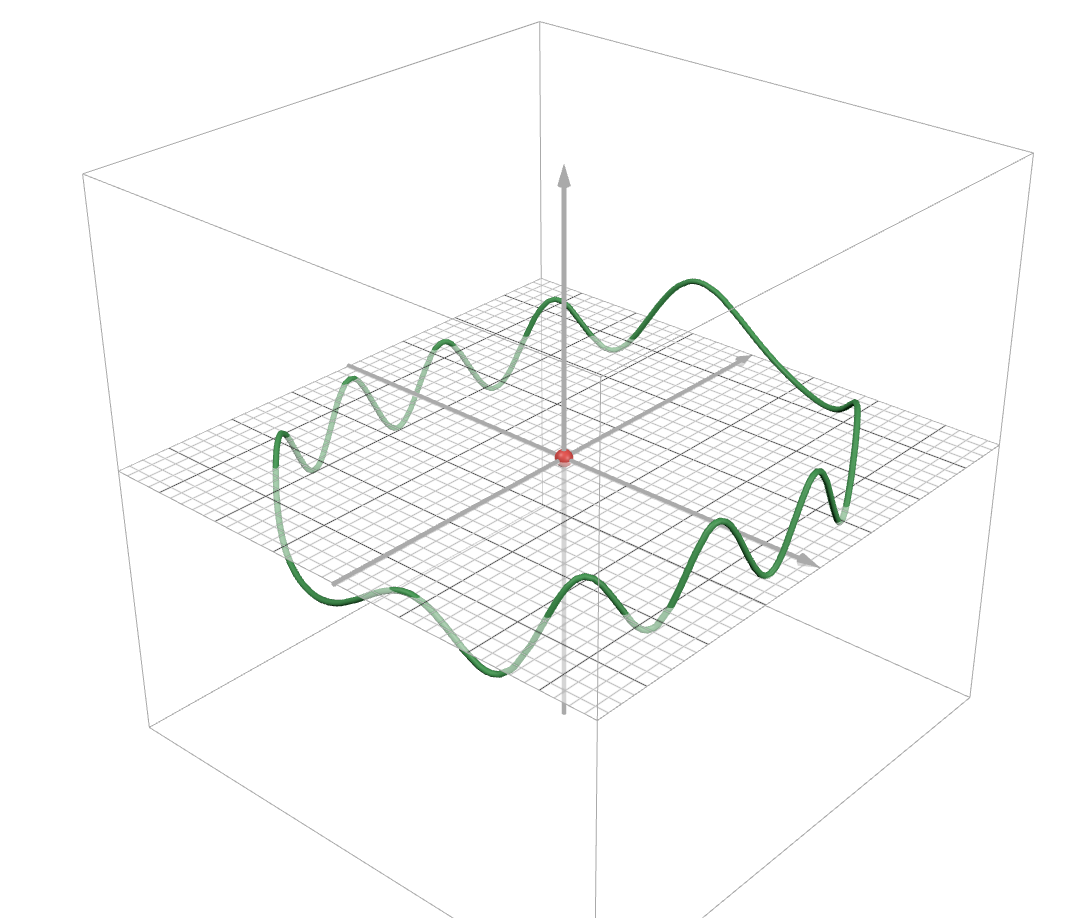
\includegraphics[width=\linewidth]{images/3d-conversion-of-trial.png}
      \captionof{figure}{3D toroidal curve in the prototype environment}
    \end{column}
  \end{columns}
\end{frame}

% ── 10  Curve Equation ──────────────────────────────
\begin{frame}{Toroidal Curve Equation: Porting from 2D to 3D}
  \begin{block}{Mathematical Foundation}
    \vspace{0.5em}
    The curve is defined on a toroidal surface by combining a circular cross-section with a sinusoidal height component:
    { \tiny
      \begin{align*}
        &x^2 + y^2 = r^2 \\
        &z = \sum_{i=1}^{3} \left[ \alpha_i \sin(\omega_i \theta) + \beta_i \cos(\omega_i \theta) \right]
      \end{align*}
    }
    {\small where $\alpha_1, \alpha_2, \alpha_3$ and $\beta_1, \beta_2, \beta_3$ are the \textbf{6 adjustable coefficients} that control curve complexity.}
  \end{block}

  \vspace{0.3em}
  \begin{columns}[T]
    \begin{column}{0.48\textwidth}
      \centering
      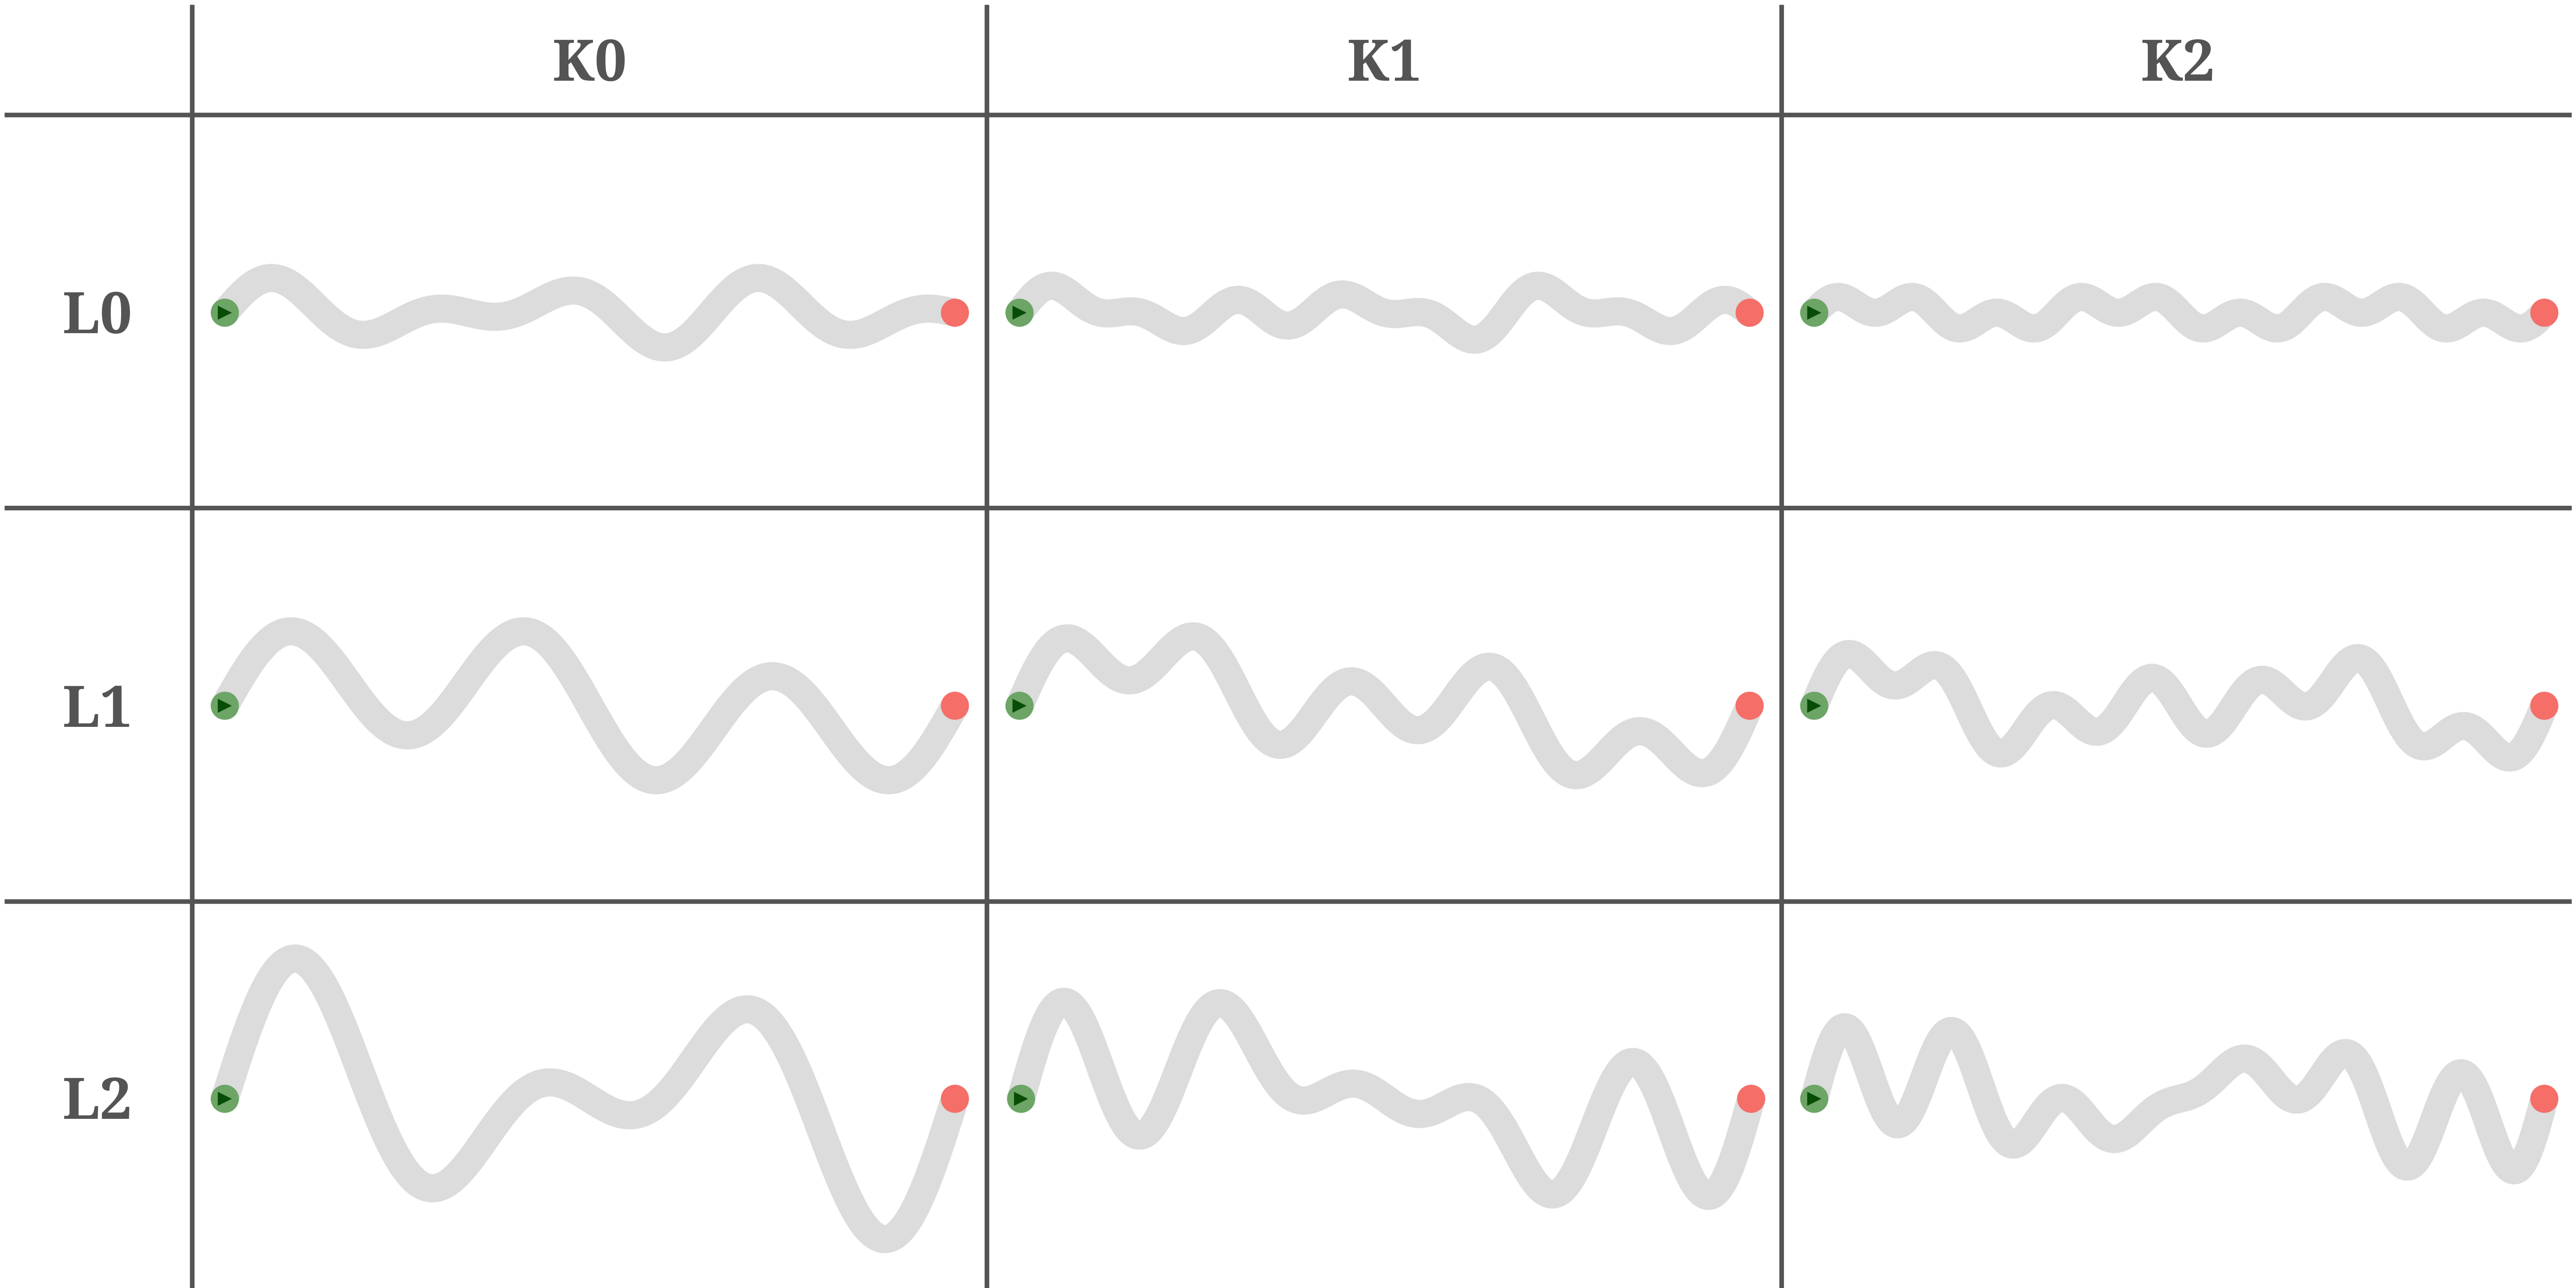
\includegraphics[width=0.85\linewidth]{images/path_diagram.png}
      \captionof{figure}{2D path (Chen et al.)}
    \end{column}
    \begin{column}{0.48\textwidth}
      \centering
      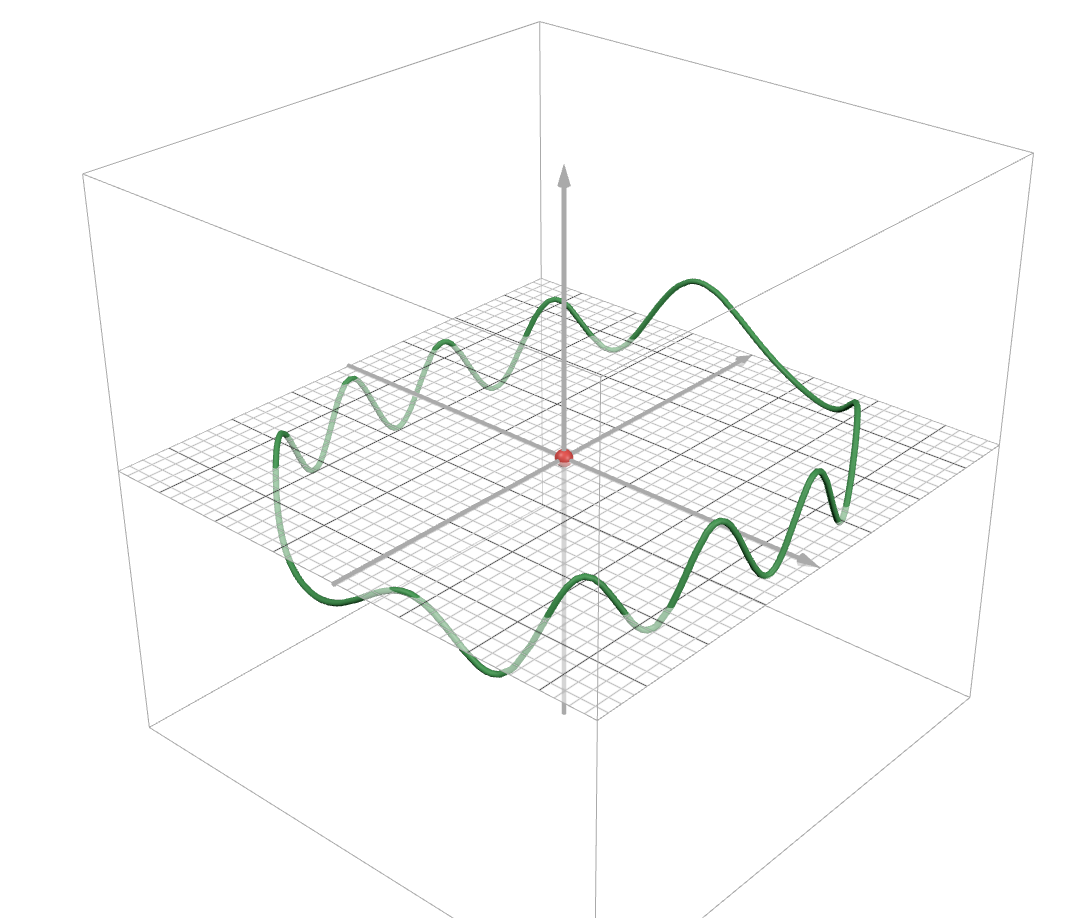
\includegraphics[width=0.5\linewidth]{images/3d-conversion-of-trial.png}
      \captionof{figure}{3D toroidal conversion}
    \end{column}
  \end{columns}
\end{frame}

% ━━━━━━━━━━━━━━━━━━━━━━━━━━━━━━━━━━━━━━━━━━━━━━━━━
\section{Prototype Design Methodology}
% ━━━━━━━━━━━━━━━━━━━━━━━━━━━━━━━━━━━━━━━━━━━━━━━━━

% ── 11  Design Process ──────────────────────────────
\begin{frame}{Design Methodology}
  \begin{columns}[T]
    \begin{column}{0.48\textwidth}
      \textbf{Prototyping Approach}
      \begin{enumerate}
        \item \textbf{Requirements Analysis} (Assignment 1)\\
              Personas, scenarios, functional requirements
        \item \textbf{Conceptual Sketching}\\
              Wireframes for curve display and control UI
        \item \textbf{High-Fidelity Prototyping}\\
              Direct implementation in Unity3D
        \item \textbf{Iterative Refinement}\\
              Testing curve trackability and data export
      \end{enumerate}
    \end{column}
    \begin{column}{0.48\textwidth}
      \textbf{Tools \& Technologies}
      \begin{itemize}
        \item \textbf{Engine:} Unity3D (C\#)
        \item \textbf{Curve Rendering:} Procedural mesh generation on torus
        \item \textbf{Input:} Mouse-based dragging (desktop)
        \item \textbf{Data Export:} CSV with timestamps
        \item \textbf{Target Platform:} Windows 10+ (desktop)
      \end{itemize}

      \vspace{0.5em}
      \textbf{No AI Behaviour Simulation}\\
      The prototype is a \emph{data collection tool}; it does not simulate AI responses. AI/ML analysis is a downstream task performed on the exported data.
    \end{column}
  \end{columns}
\end{frame}

% ━━━━━━━━━━━━━━━━━━━━━━━━━━━━━━━━━━━━━━━━━━━━━━━━━
\section{Prototype Artifacts \& Interface Design}
% ━━━━━━━━━━━━━━━━━━━━━━━━━━━━━━━━━━━━━━━━━━━━━━━━━

% ── 12  Wireframes ──────────────────────────────────
\begin{frame}{Wireframes (1/2)}
  \begin{columns}[T]
    \begin{column}{0.48\textwidth}
      \textbf{Frame 1}
      \begin{center}
        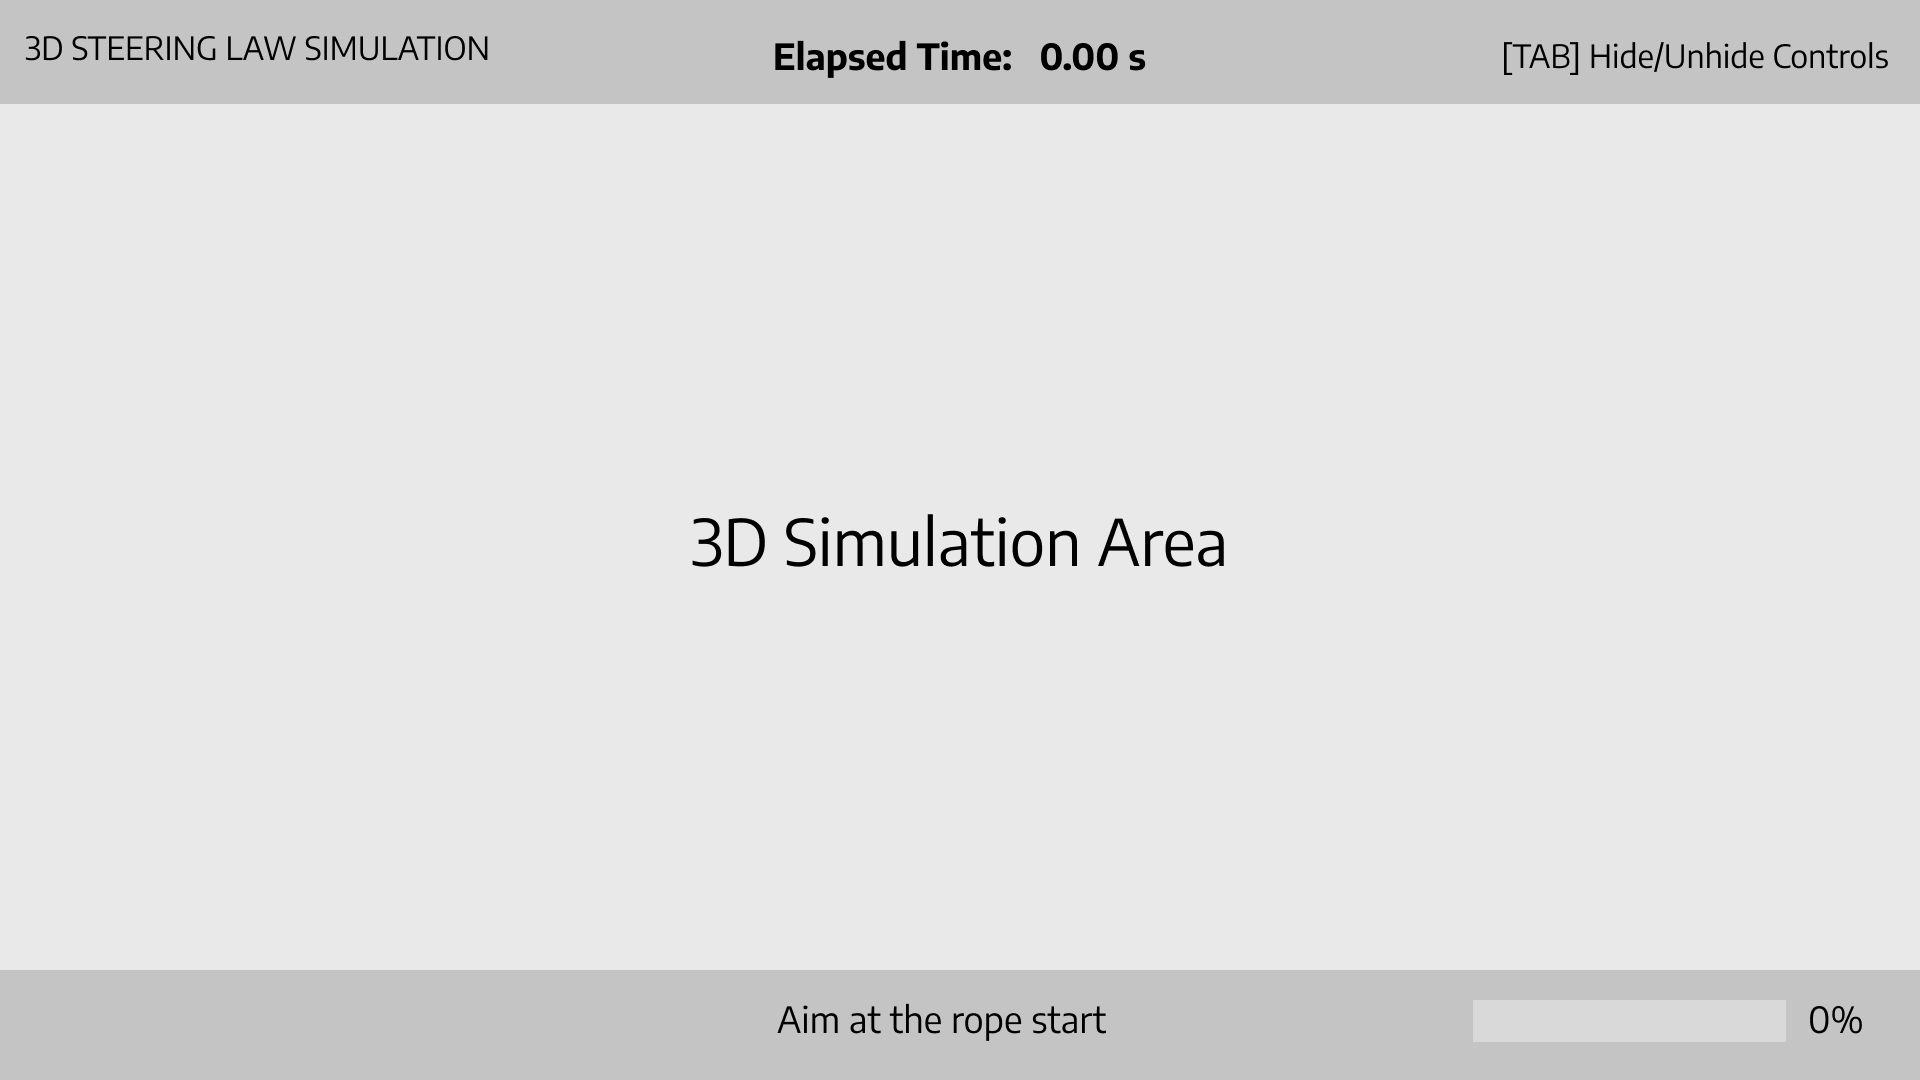
\includegraphics[width=\linewidth]{Wireframes/Frame1.png}
      \end{center}
    \end{column}
    \begin{column}{0.48\textwidth}
      \textbf{Frame 2}
      \begin{center}
        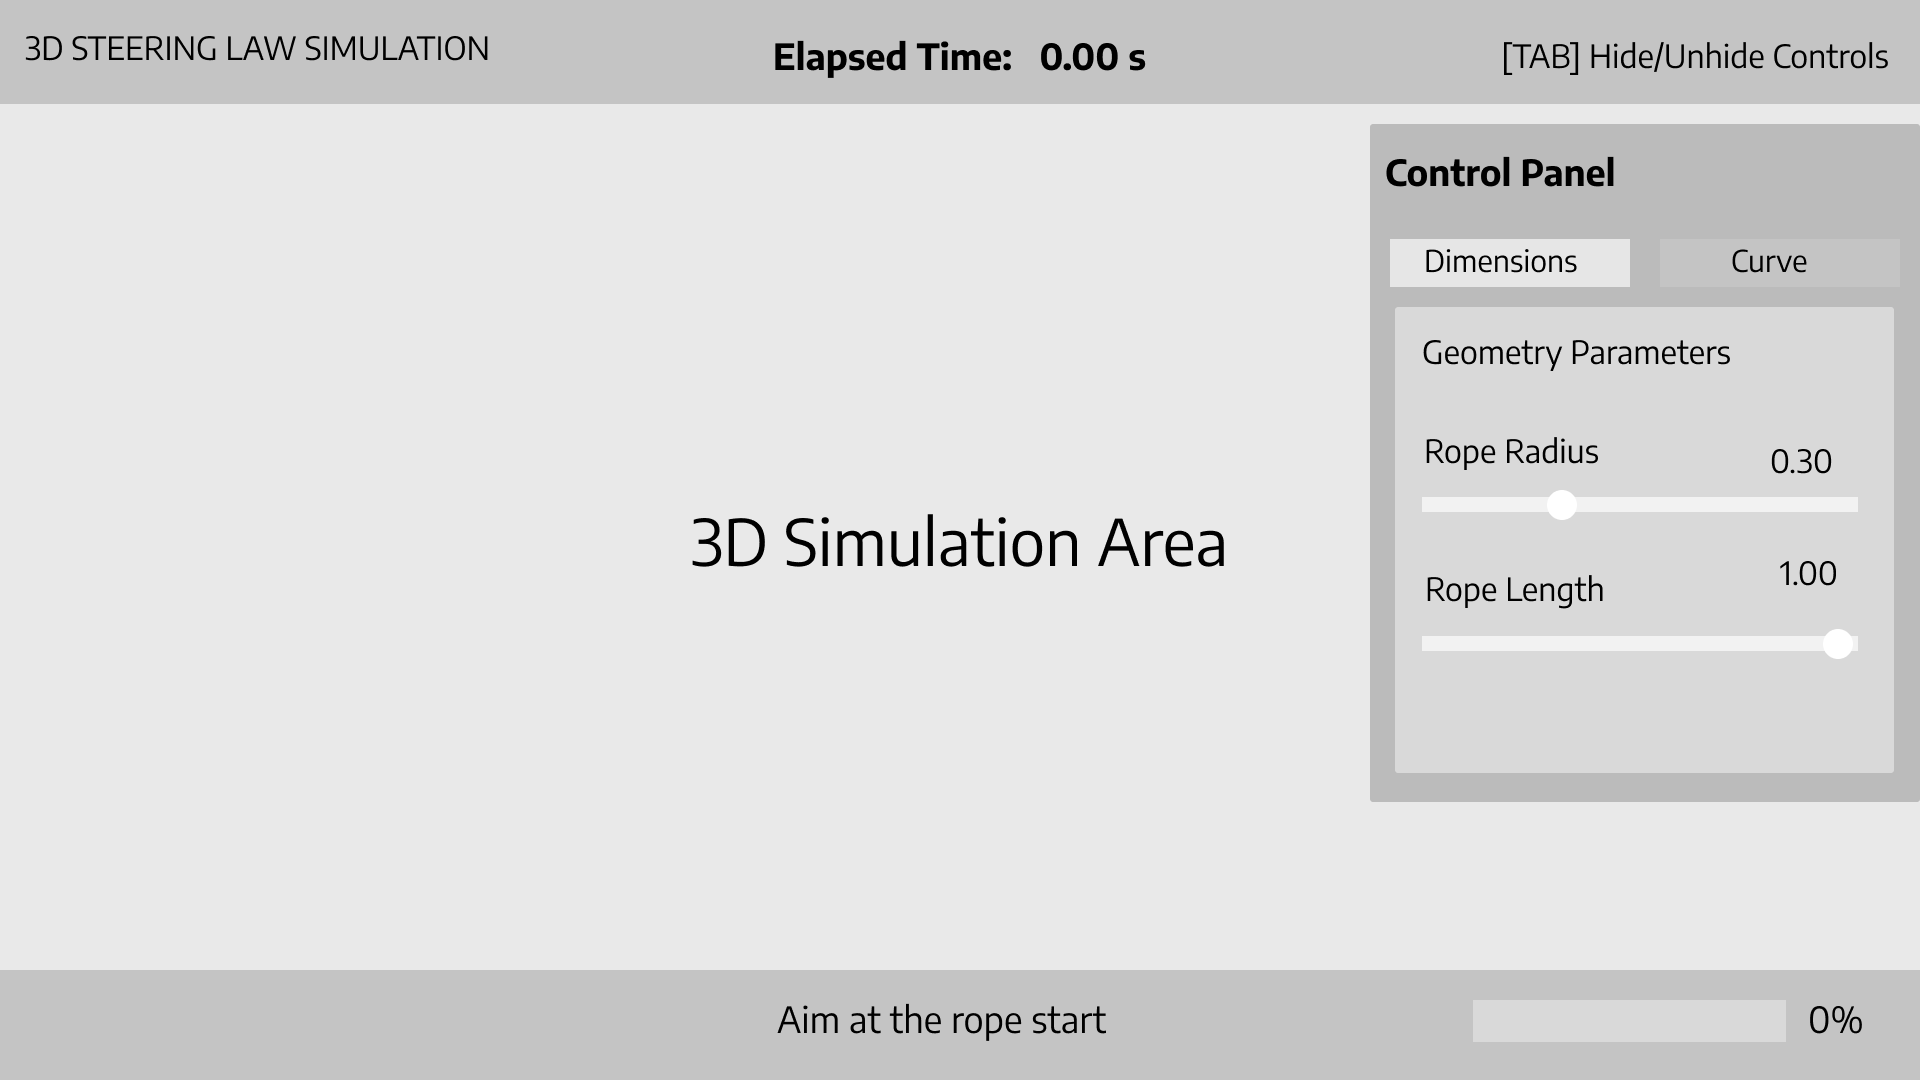
\includegraphics[width=\linewidth]{Wireframes/Frame2.png}
      \end{center}
    \end{column}
  \end{columns}
\end{frame}

\begin{frame}{Wireframes (2/2)}
  \begin{columns}[T]
    \begin{column}{0.48\textwidth}
      \textbf{Frame 3}
      \begin{center}
        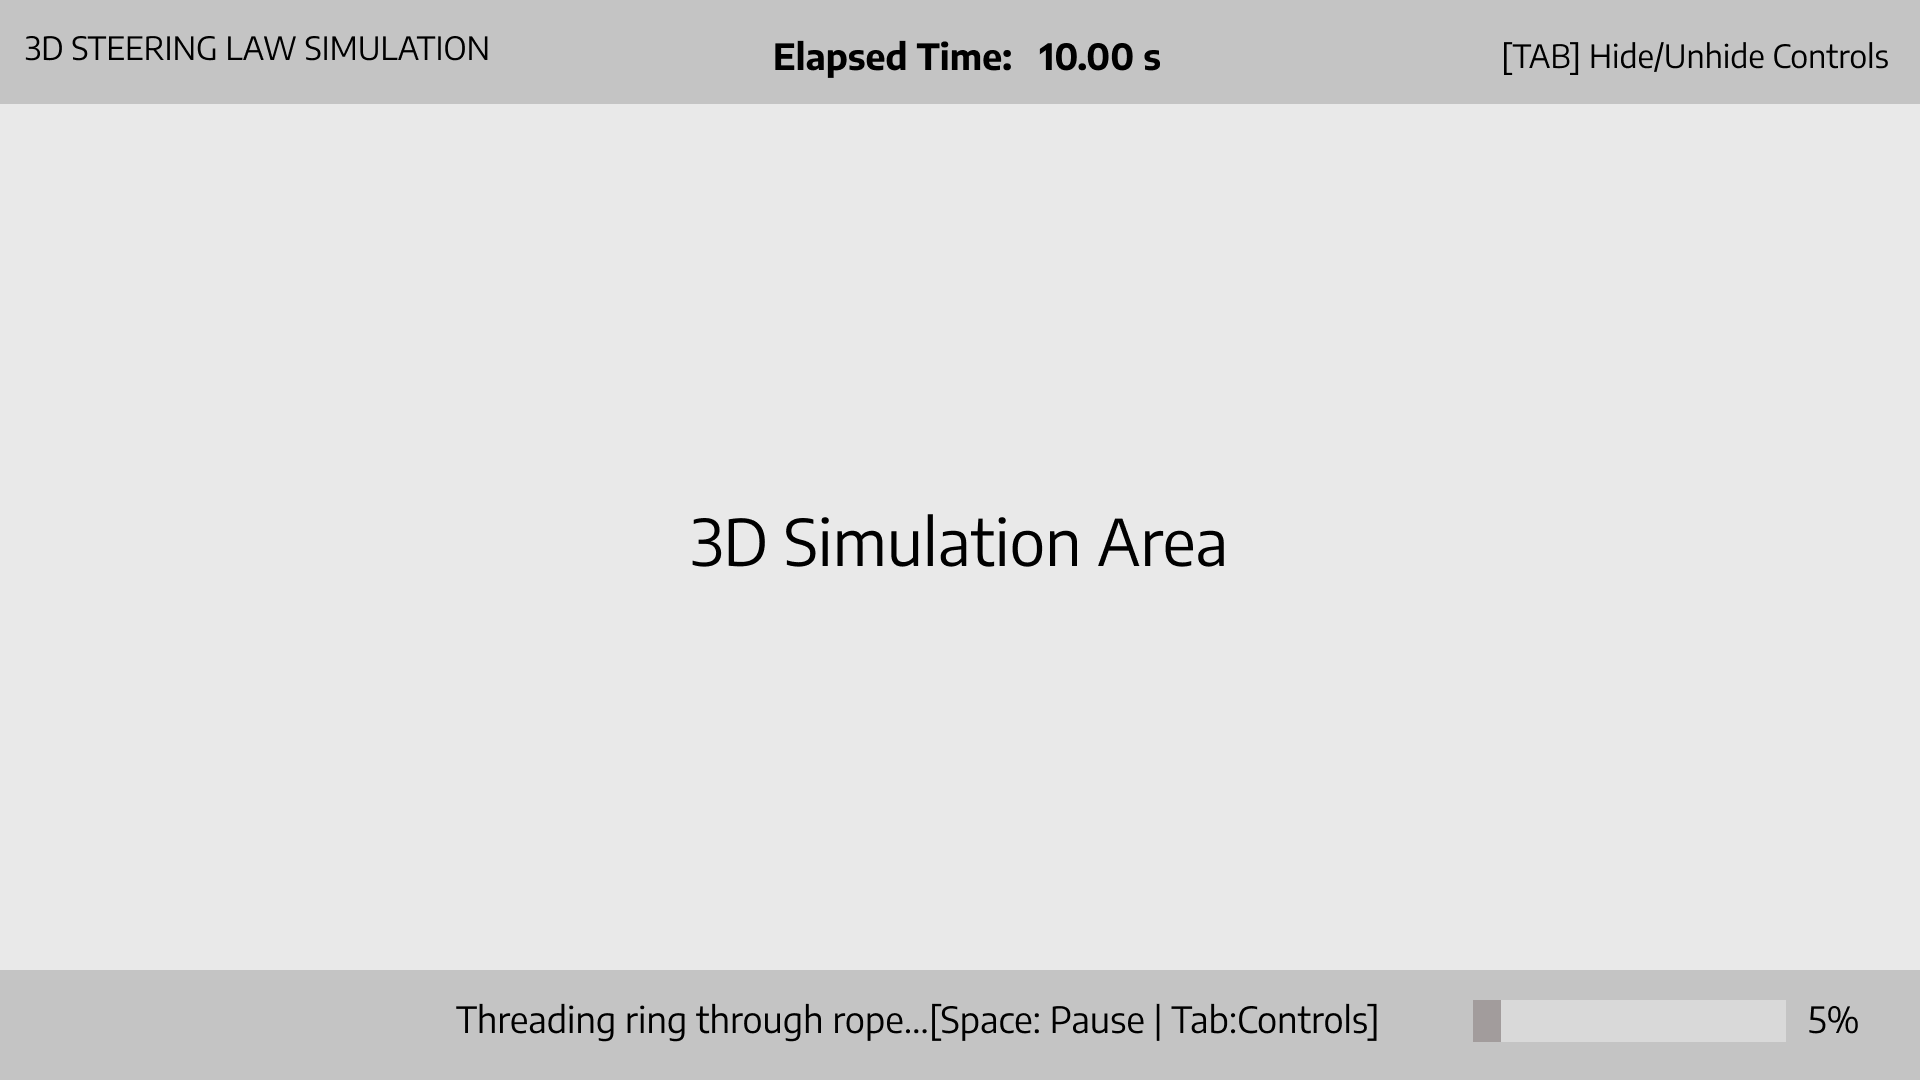
\includegraphics[width=\linewidth]{Wireframes/Frame3.png}
      \end{center}
    \end{column}
    \begin{column}{0.48\textwidth}
      \textbf{Frame 4}
      \begin{center}
        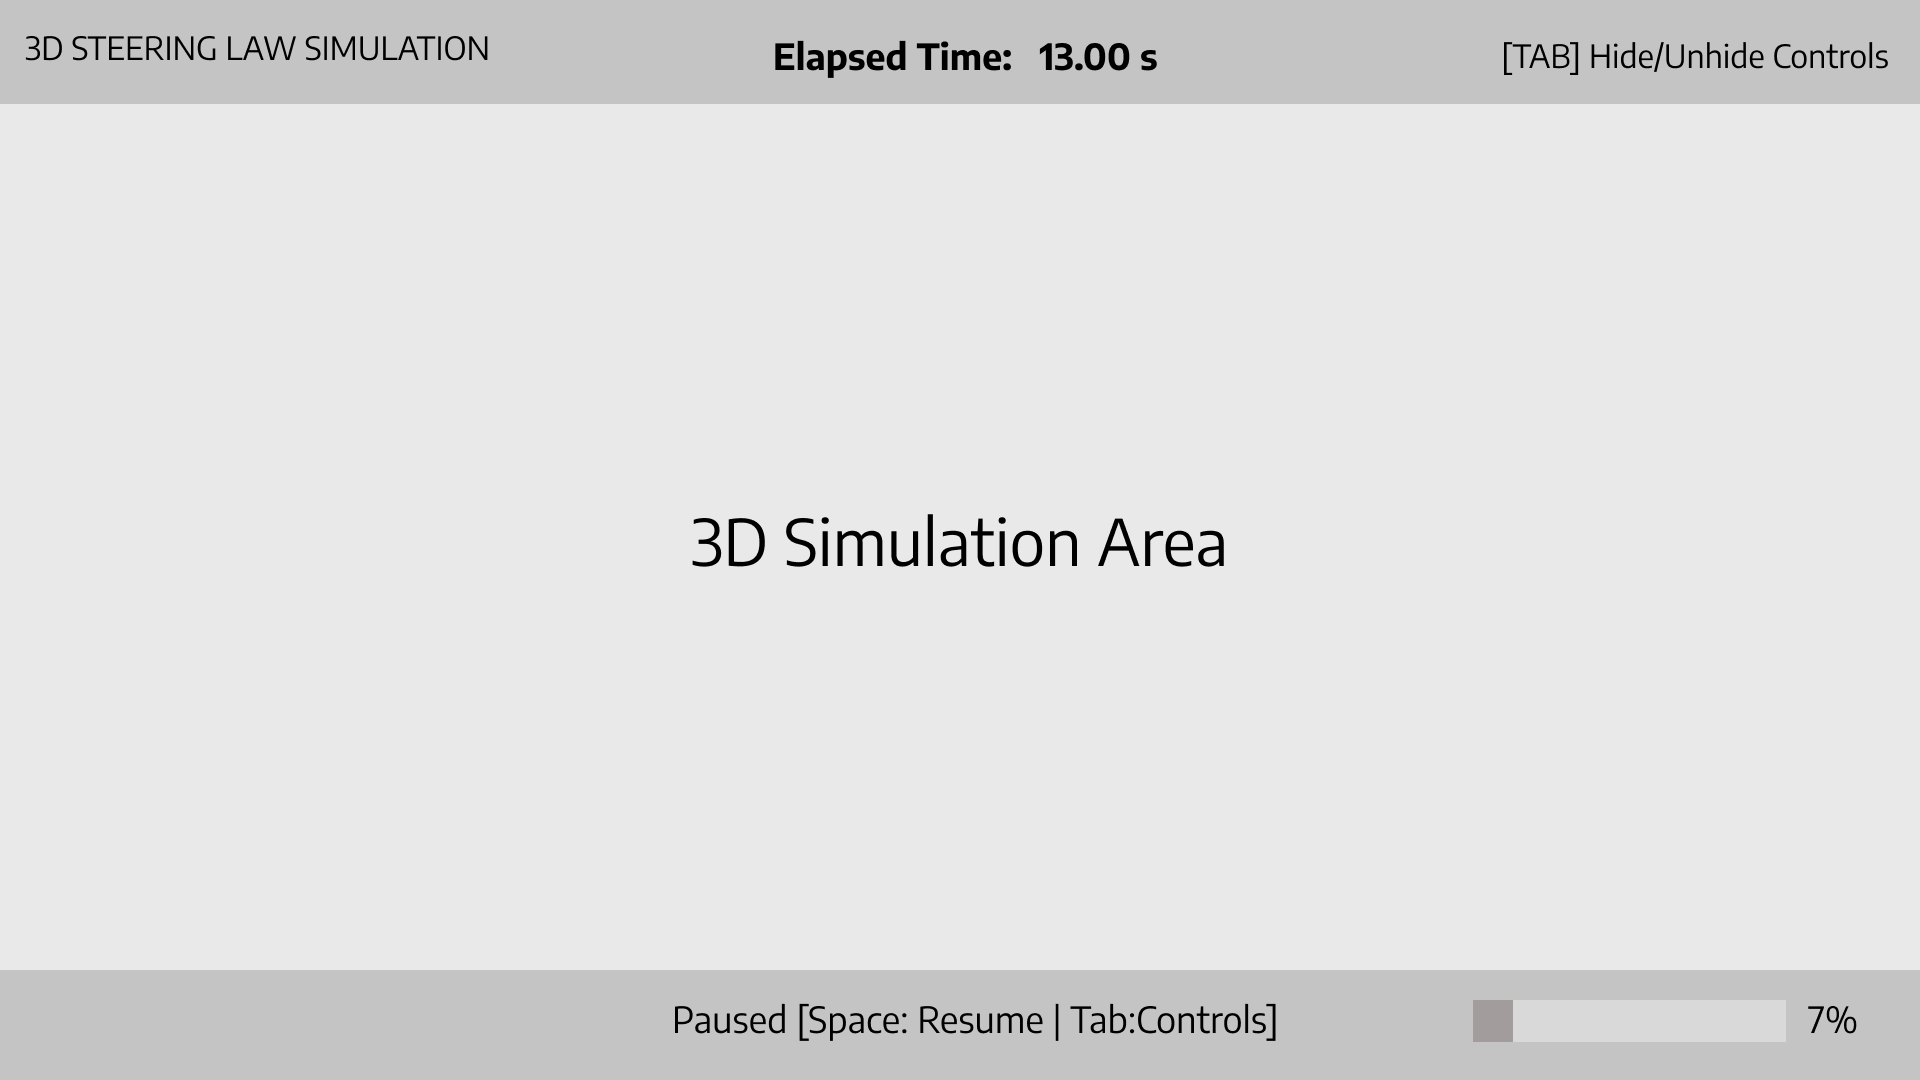
\includegraphics[width=\linewidth]{Wireframes/Frame4.png}
      \end{center}
    \end{column}
  \end{columns}
\end{frame}

% ── 13  Interface Screens ───────────────────────────
\begin{frame}{Interface Screens (1/3)}
  \begin{columns}[T]
    \begin{column}{0.48\textwidth}
      \textbf{Curve}
      \begin{center}
        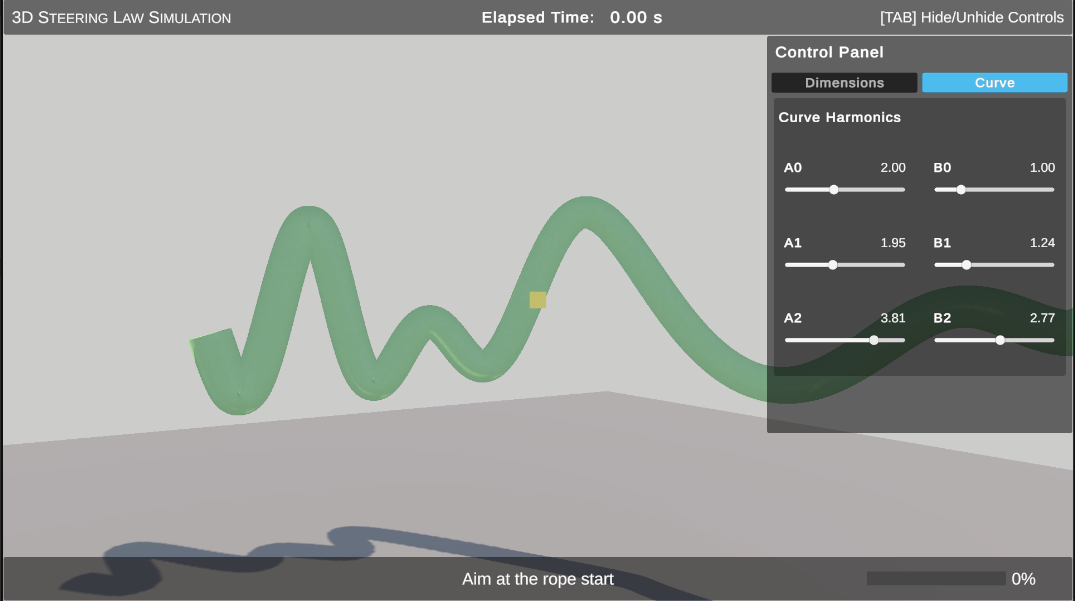
\includegraphics[width=\linewidth]{UserInterface/Curve.png}
      \end{center}
    \end{column}
    \begin{column}{0.48\textwidth}
      \textbf{Paused}
      \begin{center}
        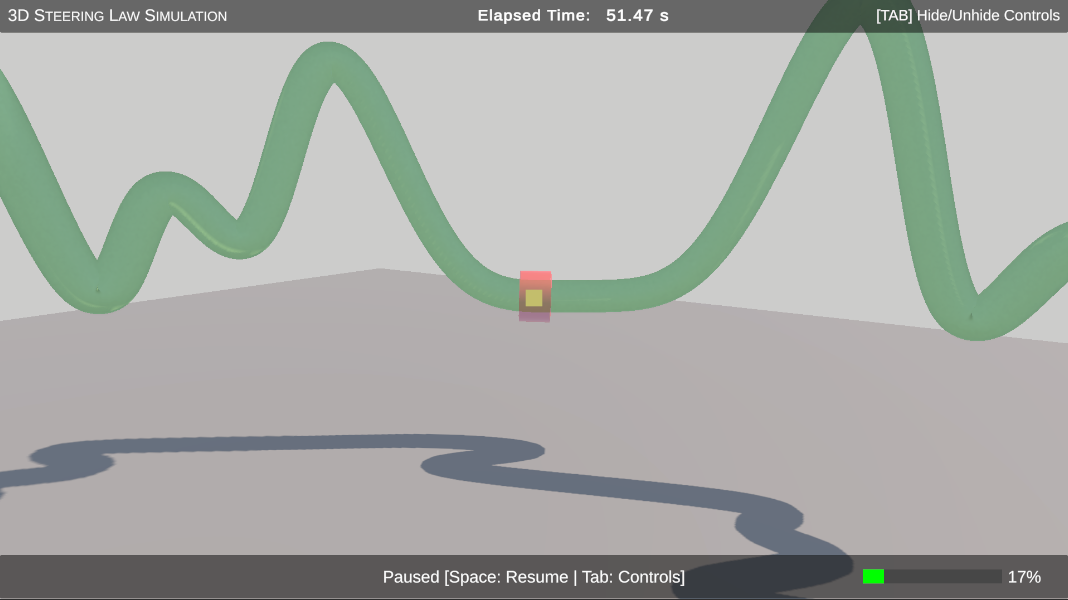
\includegraphics[width=\linewidth]{UserInterface/Paused.png}
      \end{center}
    \end{column}
  \end{columns}
\end{frame}

\begin{frame}{Interface Screens (2/3)}
  \begin{columns}[T]
    \begin{column}{0.48\textwidth}
      \textbf{Radius adjustment}
      \begin{center}
        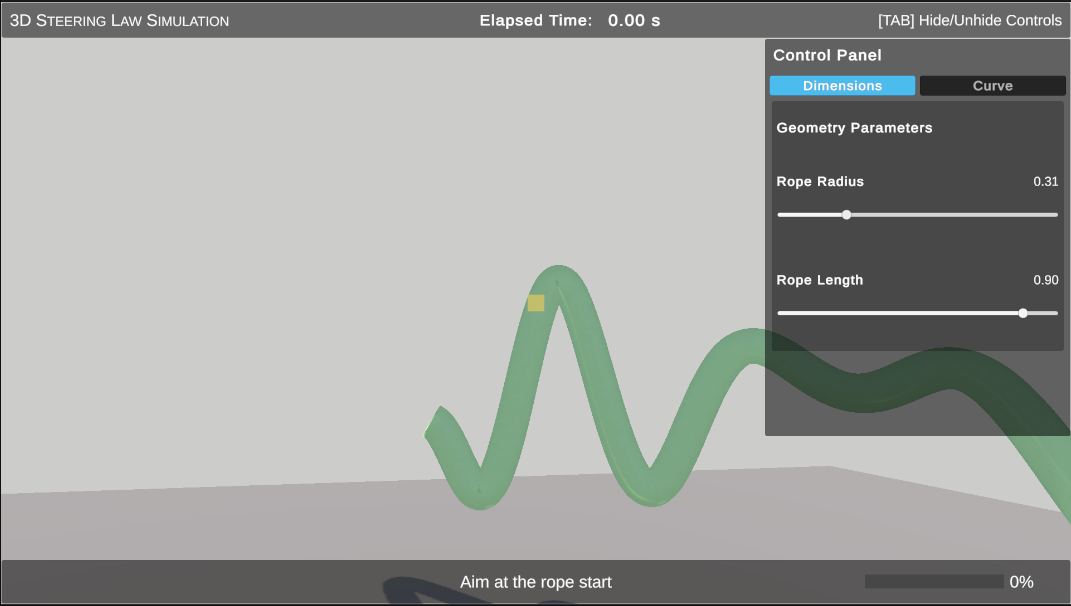
\includegraphics[width=\linewidth]{UserInterface/Radius.png}
      \end{center}
    \end{column}
    \begin{column}{0.48\textwidth}
      \textbf{Start of task}
      \begin{center}
        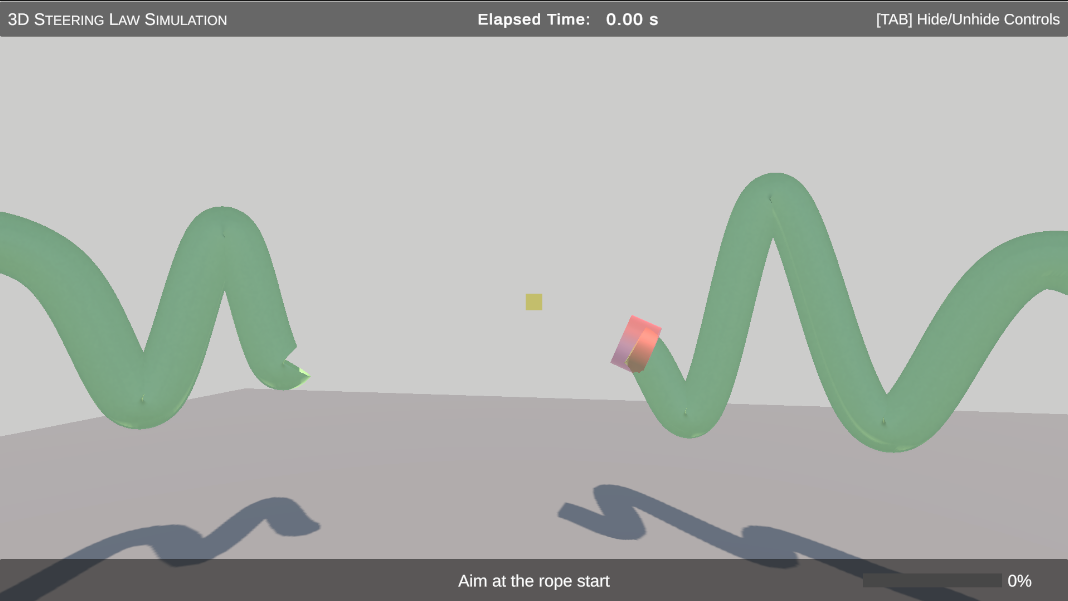
\includegraphics[width=\linewidth]{UserInterface/Start.png}
      \end{center}
    \end{column}
  \end{columns}
\end{frame}

\begin{frame}{Interface Screens (3/3)}
  \begin{columns}[T]
    \begin{column}{0.48\textwidth}
      \textbf{Task in progress}
      \begin{center}
        \includegraphics[width=\linewidth]{"UserInterface/Task in progress".png}
      \end{center}
    \end{column}
    \begin{column}{0.48\textwidth}
      \textbf{Task in progress with a thicker curve}
      \begin{center}
        \includegraphics[width=\linewidth]{"UserInterface/Task in progress1".png}
      \end{center}
    \end{column}
  \end{columns}
\end{frame}


% ━━━━━━━━━━━━━━━━━━━━━━━━━━━━━━━━━━━━━━━━━━━━━━━━━
\section{User Interaction \& Task Flow}
% ━━━━━━━━━━━━━━━━━━━━━━━━━━━━━━━━━━━━━━━━━━━━━━━━━

% ── 15  User Interaction ────────────────────────────
\begin{frame}{User Interaction Model}
  \begin{columns}[T]
    \begin{column}{0.48\textwidth}
      \textbf{Participant Interaction}
      \begin{enumerate}
        \item View the toroidal curve in the 3D viewport
        \item Position the crosshair at the start point
        \item \textbf{Drag along the curve} to track the toroidal path
        \item System records completion time automatically
        \item Trial ends when the end point is reached
      \end{enumerate}
    \end{column}
    \begin{column}{0.48\textwidth}
      \textbf{Experiment Setter Interaction}
      \begin{enumerate}
        \item Adjust the \textbf{6 coefficient sliders} ($\alpha_1$--$\alpha_3$, $\beta_1$--$\beta_3$)
        \item Preview the generated toroidal curve in real time
        \item Start a new trial for the participant
        \item Review exported timing data (CSV)
      \end{enumerate}

      \vspace{0.5em}
      \textbf{Input Method}\\
      Mouse-based dragging on desktop; VR controller input planned for future work.
    \end{column}
  \end{columns}
\end{frame}

% ── 16  Task Flow ───────────────────────────────────
\begin{frame}{Task Flow}
  \textbf{Primary Task:} \emph{Complete a 3D Toroidal Curve Tracking Trial}
  \begin{columns}[T]
    \begin{column}{0.48\textwidth}
      \begin{enumerate}
        \item \textbf{Configure Curve}\\
              Researcher sets 6 coefficients via sliders
        \item \textbf{Preview \& Validate}\\
              Visual check that the curve is well-formed and trackable
        \item \textbf{Start Trial}\\
              Participant begins dragging the crosshair along the curve
        \item \textbf{Record Data}\\
              System captures completion time with millisecond precision
        \item \textbf{Export Results}\\
              Timing data saved to CSV for analysis
      \end{enumerate}
    \end{column}
    \begin{column}{0.48\textwidth}
      \textbf{Data Captured Per Trial}
      \begin{itemize}
        \item Curve coefficients ($\alpha_1$--$\alpha_3$, $\beta_1$--$\beta_3$)
        \item Completion time (ms)
        \item Trial index and session ID
      \end{itemize}

      \vspace{0.5em}
      \textbf{No AI in the Loop}\\
      The prototype operates as a pure data collection instrument. All analysis (e.g., fitting the modified steering law model) is performed offline on the exported data.
    \end{column}
  \end{columns}
\end{frame}

% ━━━━━━━━━━━━━━━━━━━━━━━━━━━━━━━━━━━━━━━━━━━━━━━━━
\section{Implementation Details}
% ━━━━━━━━━━━━━━━━━━━━━━━━━━━━━━━━━━━━━━━━━━━━━━━━━

% ── 17  Implementation ──────────────────────────────
\begin{frame}{Implementation in Unity3D}
  \begin{columns}[T]
    \begin{column}{0.48\textwidth}
      \textbf{Platform \& Tools}
      \begin{itemize}
        \item \textbf{Engine:} Unity3D (2022 LTS or later)
        \item \textbf{Language:} C\#
        \item \textbf{Target:} Windows 10+ (desktop)
        \item \textbf{Input:} Mouse (crosshair dragging)
      \end{itemize}

      \vspace{0.5em}
      \textbf{Key Features}
      \begin{itemize}
        \item Procedural toroidal curve generation from 6 coefficients
        \item Real-time curve preview as sliders are adjusted
        \item Crosshair-based path tracking with visual feedback
        \item Millisecond-precision timer for trial duration
        \item CSV data export (coefficients + time)
      \end{itemize}
    \end{column}
    \begin{column}{0.48\textwidth}
      \textbf{Architecture}
      \begin{itemize}
        \item \textbf{CurveGenerator:} Computes toroidal mesh from coefficients
        \item \textbf{CrosshairController:} Handles user input and position tracking
        \item \textbf{TrialManager:} Manages trial lifecycle, timing, and data logging
        \item \textbf{UIManager:} Slider panel, timer display, trial controls
      \end{itemize}

      \vspace{0.5em}
      \textbf{Constraint}\\
      VR implementation (Meta Quest) is \alert{not yet implemented}; currently desktop-only with mouse input.
    \end{column}
  \end{columns}
\end{frame}

% ━━━━━━━━━━━━━━━━━━━━━━━━━━━━━━━━━━━━━━━━━━━━━━━━━
\section{Discussion \& Conclusion}
% ━━━━━━━━━━━━━━━━━━━━━━━━━━━━━━━━━━━━━━━━━━━━━━━━━

% ── 18  Alignment with Requirements ─────────────────
\begin{frame}{Alignment with Requirements (Assignment 1)}
  \small
  \begin{tabular}{@{}l p{5.8cm} l@{}}
    \toprule
    \textbf{Req.\ ID} & \textbf{Requirement} & \textbf{Status} \\
    \midrule
    FR1  & Built in Unity engine                      & \alert{Implemented} \\
    FR2  & Configurable 3D path geometry              & \alert{Implemented} \\
    FR3  & Mouse \& VR controller input               & Partial (mouse only) \\
    FR4  & Millisecond-precision timing               & \alert{Implemented} \\
    FR9  & CSV / JSON data export                     & \alert{Implemented} \\
    FR11 & Meta VR headset support                    & Not yet \\
    NFR1 & $\geq$ 60 FPS on GTX 1650                 & \alert{Met} \\
    NFR2 & Sub-perceptual input latency               & \alert{Met} \\
    \bottomrule
  \end{tabular}
\end{frame}

% ── 19  Design Trade-offs ───────────────────────────
\begin{frame}{Design Trade-offs \& Implications}
  \begin{itemize}
    \item \textbf{Data Accuracy vs.\ Visual Richness}\\
          Prioritised precise timing and consistent curves over elaborate visual design
    \item \textbf{Desktop-First vs.\ VR-First}\\
          Chose desktop (mouse) for rapid prototyping; VR integration is planned but not yet implemented
    \item \textbf{Simplicity vs.\ Feature Completeness}\\
          Focused on core data collection pipeline; advanced features (practice trials, tutorials, randomisation) deferred
    \item \textbf{Configurability vs.\ Participant Simplicity}\\
          Slider controls are exposed only to the experiment setter; participants see only the curve and crosshair
  \end{itemize}

  \vspace{0.5em}
  \alert{Design philosophy:} The prototype is an \emph{instrument for data collection}, not a polished end-user application.
\end{frame}

% ── 20  Limitations ─────────────────────────────────
\begin{frame}{Limitations}
  \begin{columns}[T]
    \begin{column}{0.48\textwidth}
      \textbf{Prototype Limitations}
      \begin{itemize}
        \item VR mode not yet implemented --- currently desktop-only
        \item No tutorial or practice trial system
        \item Limited to mouse-based input; no VR controller support
        \item No boundary violation detection yet
        \item Trial randomisation not implemented
      \end{itemize}
    \end{column}
    \begin{column}{0.48\textwidth}
      \textbf{Methodological Constraints}
      \begin{itemize}
        \item Prototype not yet evaluated with real participants
        \item Curve trackability not empirically validated across all coefficient ranges
        \item Data analysis (fitting steering law model) is offline and not part of the prototype
        \item Limited accessibility features
      \end{itemize}
    \end{column}
  \end{columns}
\end{frame}

% ── 21  Future Work ─────────────────────────────────
\begin{frame}{Future Work}
  \begin{itemize}
    \item \textbf{VR Integration:} Port the prototype to Meta Quest headsets with VR controller input
    \item \textbf{Pilot Study:} Conduct initial user studies to validate curve trackability and data quality
    \item \textbf{Extended Data Logging:} Add trajectory capture, boundary violation detection, and trial randomisation
    \item \textbf{Steering Law Fitting:} Analyse collected data to evaluate the modified Fitts' law in 3D
    \item \textbf{Accessibility:} Add pause/resume, fatigue-aware breaks, and adjustable tolerances
    \item \textbf{ML Analysis Pipeline:} Build downstream tools for outlier detection, movement time prediction, and interpretable models
  \end{itemize}
\end{frame}

% ── 22  Conclusion ──────────────────────────────────
\begin{frame}{Conclusion}
  \begin{itemize}
    \item Designed and constructed a \textbf{high-fidelity Unity3D prototype} for studying
          human steering performance on complex 3D toroidal curves
    \item The curve is defined by \textbf{6 adjustable coefficients} (3 sine + 3 cosine),
          enabling systematic variation of path complexity
    \item Users track the curve via a \textbf{crosshair-based dragging interaction};
          the system records completion time with millisecond precision
    \item The prototype is grounded in \textbf{HCAI principles}: transparency,
          human oversight, and reproducibility
    \item Provides the foundation for \textbf{empirical evaluation} of the steering law
          on 3D curved trajectories
  \end{itemize}

  \vspace{1em}
  \centering
  {\Large\bfseries Thank You!}\\[0.3em]
  Questions?
\end{frame}

% ── References ──────────────────────────────────────
\begin{frame}[allowframebreaks]{References}
  \printbibliography[heading=none]
\end{frame}

\end{document}
